
\documentclass[hidelinks,12pt]{article}
\usepackage{minted}
\usepackage[utf8]{inputenc}
\usepackage{tikz}
\usetikzlibrary{shapes.geometric, arrows}
\usepackage[utf8]{inputenc}
\usepackage[english]{babel}
\usepackage{titlesec}
\usepackage{hanging}
\usepackage{indentfirst}
\usepackage{setspace}
\usepackage{float}
\usepackage{multirow}
\usepackage{mathrsfs}
\usepackage{caption}
\usepackage{tocbasic}
\usepackage[toc,page]{appendix}
\DeclareTOCStyleEntry[beforeskip=.1em plus 1pt, pagenumberformat=\textbf]{tocline}{section}
\usepackage{adjustbox}
\usepackage[english]{babel}
\setlength{\parindent}{4em}
\setlength{\parskip}{0.5em}
\usepackage{array}
\usepackage{hyperref}
\hypersetup{
    colorlinks=false,
    linkcolor=black,
    filecolor=black,
    urlcolor=black,
}
\newcommand{\MYhref}[3][blue]{\href{#2}{\color{#1}{#3}}}%
\urlstyle{same}
\usepackage[letterpaper, portrait, margin=1in]{geometry}
\usepackage{graphicx}
\graphicspath{ {images/} }
\usepackage{array}
\newcolumntype{L}[1]{>{\raggedright\let\newline\\\arraybackslash\hspace{0pt}}m{#1}}
\newcolumntype{C}[1]{>{\centering\let\newline\\\arraybackslash\hspace{0pt}}m{#1}}
\newcolumntype{R}[1]{>{\raggedleft\let\newline\\\arraybackslash\hspace{0pt}}m{#1}}

\titleclass{\subsubsubsection}{straight}[\subsection]

\newcounter{subsubsubsection}[subsubsection]
\renewcommand\thesubsubsubsection{\thesubsubsection.\arabic{subsubsubsection}}

\titleformat{\subsubsubsection}
  {\normalfont\normalsize\bfseries}{\thesubsubsubsection}{1em}{}
\titlespacing*{\subsubsubsection}
{0pt}{3.25ex plus 1ex minus .2ex}{1.5ex plus .2ex}

\makeatletter
\renewcommand\paragraph{\@startsection{paragraph}{5}{\z@}%
  {3.25ex \@plus1ex \@minus.2ex}%
  {-1em}%
  {\normalfont\normalsize\bfseries}}
\renewcommand\subparagraph{\@startsection{subparagraph}{6}{\parindent}%
  {3.25ex \@plus1ex \@minus .2ex}%
  {-1em}%
  {\normalfont\normalsize\bfseries}}
\def\toclevel@subsubsubsection{4}
\def\toclevel@paragraph{5}
\def\toclevel@paragraph{6}
\def\l@subsubsubsection{\@dottedtocline{4}{7em}{4em}}
\def\l@paragraph{\@dottedtocline{5}{10em}{5em}}
\def\l@subparagraph{\@dottedtocline{6}{14em}{6em}}
\makeatother

\setcounter{secnumdepth}{4}
\setcounter{tocdepth}{4}

\renewcommand{\contentsname}{Table of Contents}
\renewcommand{\listtablename}{Tables}
\renewcommand{\listfigurename}{Figures}

%========================%

\title{Creating a Graphical User Interface Given a Context Free Grammar}
\author{Finn Wander}
\date{November 2022}

\tikzstyle{startstop} = [rectangle, rounded corners, minimum width=3cm, minimum height=1cm,text centered, draw=black]
\tikzstyle{arrow} = [thick,->,>=stealth]

\makeatletter
\AtBeginEnvironment{minted}{\dontdofcolorbox}
\def\dontdofcolorbox{\renewcommand\fcolorbox[4][]{##4}}
\makeatother

\begin{document}

\pagenumbering{gobble} % Disable page number on title page
\begin{center}
    \Huge{\textbf{Graphical User Interface Generation From Context Free Grammars}} \\ % Input title of MQP
    \vspace{10mm} % Add vertical space between sections
    \large{
    A Major Qualifying Project (MQP) Report \\
    Submitted to the Faculty of \\
    WORCESTER POLYTECHNIC INSTITUTE \\
    in partial fulfillment of the requirements \\
    for the Degree of Bachelor of Science in \\
    } % Do not edit this portion
    \Large{
    \vspace{5mm} % Add vertical space between sections
    Computer Science, \\ % Input first major
    \vspace{10mm} % Add vertical space between sections
    By: \\
    \vspace{5mm} % Add vertical space between sections
    Finn Wander \\ % Input first author name
    \vspace {25mm} % Add vertical space between sections
    Project Advisors: \\ % Edit if only one advisor
    \vspace{5mm} % Add vertical space between sections
    Garry Pollice \\ % Input name of first advisor
    \vspace {20mm} % Add vertical space between sections
    Date: Feb 2023 \\ % Input date of project submission
    }
    \vspace{10mm} % Add vertical space between sections
    \large{\textit{This report represents work of WPI undergraduate students submitted to the faculty as evidence of a degree requirement. WPI routinely publishes these reports on its website without editorial or peer review. For more information about the projects program at WPI, see \url{http://www.wpi.edu/Academics/Projects}.}} % Do not edit this portion
\end{center}


\newpage % Start new page
\pagenumbering{roman} % Set page numbering to lower case Roman numerals (Use 'Roman' for capital Roman numerals)
\setcounter{page}{1} % Set page number to 1

\section*{Abstract} % Start the section 'Abstract'. Include the asterisks to keep section unnumbered and off of the table of contents

\noindent Type abstract here. % Use '\noindent' to remove indentation from the first paragraph of each section
\par Second paragraph of abstract % Use '\par' to start a new paragraph

\newpage % Start new page
\section*{Acknowledgements} % Start the section 'Acknowledgements'. Include the asterisks to keep section unnumbered and off of the table of contents

\noindent Begin list of acknowledgements
\begin{enumerate} % Start a numbered list
    \item First Acknowledgement % Name of first acknowledgement
    \item Second Acknowledgement % Add new item with '\item'
\end{enumerate}

% OR %

\begin{itemize} % Start a bulletted list
    \item First Acknowledgement % Name of first acknowledgement
    \item Second Acknowledgement % Add new item with '\item'
\end{itemize}

\newpage % Start new page 
\tableofcontents % Table of contents
\listoftables % List of tables
\listoffigures % List of figures

\newpage % Start new page
\begin{doublespacing} % Adjust spacing
\pagenumbering{arabic} % Set page numbering to Arabic numbers
\setcounter{page}{1} % Set page number to 1


\section{Introduction}

Creating responsive user interfaces can be a challenging and time-consuming task. To simplify this process, many tools have been developed to generate user interfaces automatically based on developer input. However, these tools often lack the flexibility necessary to support input formats that can be described as context-free grammars.

There are many software tools that use context free grammars as input. For example ANTLR generates a parser given a context free grammar as input. This idea is very natural when dealing with syntax for languages. This MQP examines extending this idea from parser generators to UI generators. This MQP developed a tool for creating graphical user interfaces that allow user input to define a valid program of a given context free grammar. Along with this tool, this MQP implemented uses for this UI generator, including a LLVM learning tool and a lambda calculus interpreter.

UIG, or User Interface Generator, is a tool that allows programmers to input a context-free grammar in EBNF form and generate a user interface that lets web users build an abstract syntax tree based on that grammar. The tool generates fully functional web interfaces based on the syntax tree created by the web user and also generates Visitor classes that allow programmers to traverse the AST given by the user. UIG can handle any context-free grammar and even a more powerful superset of context-free grammars by allowing programmers to specify that a terminal symbol on the right-hand side of a rule refers to a previously defined instance of that symbol. UIG provides an easy way to create custom and complex user interfaces for the web.

This MQP was originally set out to address a critical lack of beginner friendly documentation of LLVM IR Builder. This MQP investigated the current state of resources for learning LLVM IR Builder and identified opportunities for improvement. It also examined existing tools and resources that are available for learning the LLVM IR Builder, and explored the challenges that students could be facing as they are learning this technology.

The UI generator was used to create a tool for learning LLVM IR generation using principals from object oriented design patterns. The expected result was a web application that guides the user through several common code generation patterns. These patterns react to user input in order to generate appropriate examples of LLVM IRBuilder usage. The patterns serve as pieces of important code that each communicate a key piece of understanding LLVM IR. Importantly the output of the application contains links to other patterns that are used in patterns that rely on each other. With each pattern there are also sections describing when, why, and how they should be used. This report will cover basic concepts of LLVM IR in order to lay out context for these patterns.

Given this context for the project, the background section will cover concepts of LLVM and its IR Builder. The background section will also discuss Lambda calculus, context-free grammars, user interface generation builders, and the technologies used in this project. In the methodology section, we will discuss the timeline of the project, and we will explore the features of UIG in more detail; covering its grammar input and user interface generation capabilities, as well as its Visitor classes and AST traversal functionality. In the results section. We will discuss the results of the useability tests. Then we'll examine the benefits of using UIG for web development through the lens of the two tools this MQP created with it.

\section{Background}
\subsection{Domain Specific Languages}
\subsection{LLVM}
Modern applications are complex, large, and written in multiple languages, which calls for program analysis and transformation throughout the program's lifetime. LLVM is a compiler framework that aims to make lifelong program analysis and transformation available for arbitrary software in a transparent manner. LLVM achieves this through two parts: (a) a code representation with several novel features that serves as a common representation for analysis, transformation, and code distribution; and (b) a compiler design that exploits this representation to provide a combination of capabilities that is not available in any previous compilation approach. 
\cite{lattner_llvm_2004}

The LLVM code representation describes a program using an abstract RISC-like instruction set but with key higher-level information for effective analysis, including type information, explicit control flow graphs, and an explicit dataflow representation. LLVM is source-language-independent, using a low-level instruction set and memory model that are only slightly richer than standard assembly languages. The LLVM compiler framework exploits the code representation to provide a combination of five capabilities that are important to support lifelong analysis and transformation for arbitrary programs, including persistent program information, offline code generation, user-based profiling and optimization, transparent runtime model, and machine-level concurrency support.
\cite{lattner_llvm_2004}

The initial reason this UI generator was created was to serve as the front-end for a tool for learning about LLVM IR Builder. LLVM is a useful tool that has been adopted by many prominent software projects such as rustc and clang. However, the use of LLVM can be challenging for students who are new to this technology. In particular, the LLVM IR Builder, a component of LLVM that is responsible for generating the intermediate representation of the source code, can be difficult to understand and use effectively due to a lack of clear documentation.

\subsubsection*{Where Does LLVM IR Fit Into A Compiler}
In the three phase approach to compiler design there is a front-end, middle-end, and back-end. The front-end handles parsing and translating to an intermediate representation. The middle-end, makes a number of optimization passes on the IR to improve the output code's performance. The back-end, transforms IR to produce machine code optimized for a particular target platform. LLVM also makes use of IR for a collection of libraries and tools that can be used for tasks like link-time optimization, debugging, and profiling.

It is important to note that LLVM does not provide tooling for creating a front-end. Creating an abstract syntax tree and lowering it to LLVM IR is up to the user of the LLVM tool chain. 

\begin{figure}[ht]
    \centering
    \caption{Front-end of a compiler}
        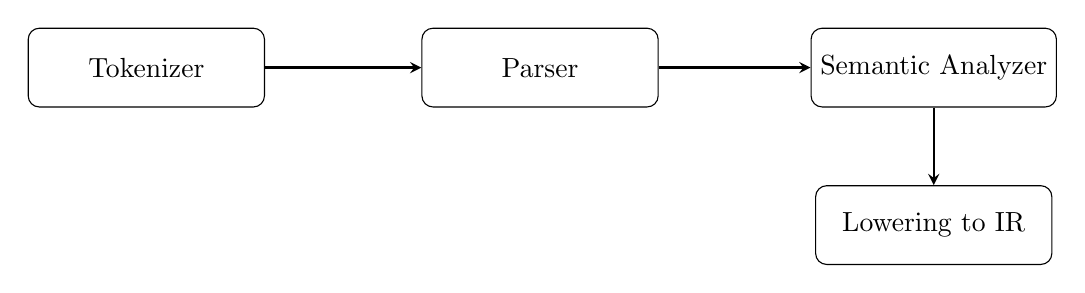
\begin{tikzpicture}[node distance=2cm]
        \node (tok) [startstop] {Tokenizer};
        \node (parse) [startstop, right of=tok, xshift=3cm] {Parser};
        \node (be) [startstop, right of=parse, xshift=3cm] {Semantic Analyzer};
        \node (ir) [startstop, below of=be] {Lowering to IR};
        
        \draw [arrow] (tok) -- node[anchor=north] {} (parse);
        \draw [arrow] (parse) -- node[anchor=north] {} (be);
        \draw [arrow] (be) -- node[anchor=north] {} (ir);
        \end{tikzpicture}
    \label{fig:front-end}
\end{figure}

\begin{figure}[ht]
    \centering
    \caption{LLVM code generation phases}
        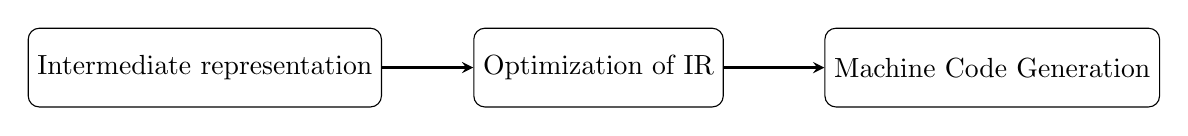
\begin{tikzpicture}[node distance=2cm]
        \node (fe) [startstop] {Intermediate representation};
        \node (op) [startstop, right of=fe, xshift=3cm] {Optimization of IR};
        \node (be) [startstop, right of=op, xshift=3cm] {Machine Code Generation};
        
        \draw [arrow] (fe) -- node[anchor=north] {} (op);
        \draw [arrow] (op) -- node[anchor=north] {} (be);
        \end{tikzpicture}
    \label{fig:LLVM diagram}
\end{figure}

\vspace{1cm}
Depending on the goals of the user of LLVM, the user could be involved in any of these steps. For example, if a user designed their own cpu they would be defining their own instruction set for LLVM to optimize and compiler to. The type of user the tool this project focuses on are users primarily concerned with translating their AST into IR. 

\subsubsection{LLVM Instruction Set}
The LLVM instruction set is designed to represent programs in a way that supports advanced analyses and transformations while allowing for extensive optimization in static compilers. The instruction set is based on an infinite set of typed virtual registers that can hold values of primitive types. The instruction set includes only 31 opcodes, and most instructions are in three-address form, taking one or two operands and producing a single result.
\cite{noauthor_llvm_2023}

\subsubsection{LLVM IR and IR Builder}
LLVM IR is a virtual instruction set That can be represented in 3 forms: plain-text, binary, and in-memory. The plain-text representation is based on a human-readable syntax, while the binary representation is a more compact form used for storage and transmission. The in-memory representation is used for optimization and analysis, and it is designed to be both efficient and flexible.
\cite{noauthor_llvm_2023}

?TODO expand on Human readable form 
?TODO insert listing for IR assebily

LLVM has a collection of classes that are used to represent modules, functions, basic blocks, and instructions in IR, this is the "in program memory" representation of IR. For example the AllocaInst object represents an alloca instruction in IR, this makes space the stack for a given type and returns a pointer to that space for you. To create an alloca instruction in a program, you could either create the AllocaInst object and then add it in the correct location of a basic block object, that you've already added to a function object, that you've already added to a Module object, or, you could use the IR Builder to manage all of that for you. The IR Builder class keeps track of where it is adding instructions and then exposes an interface that lets you make a call to CreateAlloca(). This creates an alloca instruction for you in a program at the location after you've last inserted an instruction.

\subsubsection*{Context and Module}

LLVm provides a class that stores 

\subsubsection*{Virtual Registers and Values}
IR uses virtual registers to represent values. Virtual registers provide a more abstract representation of values than hardware registers in two ways. 1; they can represent aggregate types such as structs or arrays. 2; there is an unbounded amount of them. 

Virtual registers are used in LLVM to facilitate the implementation of Single Static Assignment (SSA) form. SSA is a representation of a program in which each variable is assigned exactly once. Unique virtual register names are required due to SSA representation. The large number of available names solves the uniqueness problem. For example, you can name two registers \%reg.1 and \%reg.2, and they would be unique. You could also name them \%1, \%2, \%3 and so on. Virtual registers are mapped to physical registers of a target architecture. Register allocation assigns physical registers to virtual registers for optimal performance.

Every instruction in IR returns a Value*. Using the example from before, the alloca instruction returns a pointer to allocated memory. This value is then stored in a virtual register. It is important to understand that Value objects don't actually store data representing the value itself, rather, they store a representation of how that value is computed. This is evidenced by the fact that instruction objects are values. Values also take in other values as parameters, so a value becomes a nested tree of computation.
\cite{lattner_llvm_2004}
\subsubsection*{Basic Blocks and Control Flow}
In LLVM IR, a basic block is a set of instructions that are guaranteed to execute in order. There is just one entry point and one exit point for each basic block. A basic block's final instruction must be a terminator instruction like a branch, jump, return, or call. These terminating instructions are Value objects too, however usually being void typed; they represent control semantics rather than data. Because you can't have branching statements in the middle of a basic block, to achieve control constructs in LLVM you need to chain multiple of these basic blocks together. It is simpler to perform optimization and to perform register allocation when the code has been broken into these continuous, non-interrupted blocks of execution.
\cite{noauthor_llvm_2023}


In program memory, basic blocks have an object representation. They are stored in BasicBlock objects. The IR Builder can add instructions to a basic block by calling the SetInsertPoint function with a BasicBlock object. After that call, instructiions created through the IR Builder will be added to that BasicBlock. There is also a function called Create in the BasicBlock namespace that takes in a context, name, and Function object, and will return a BasicBlock pointer that belongs to that function.

\subsubsection*{Types}
Every Value object in LLVM has an associated Type object. LLVM has a type system that includes many categories. Primitive types, Void types, Function types, First-class types, Single value types, and Aggregate Types are the different categories of LLVM IR types.
\cite{noauthor_llvm_2023}
A high-level interface for creating and modifying these kinds is provided by LLVM IRBuilder. Because of the robust type system of LLVM IR, optimizations may be carried out with less analysis, leading to more effective code generation and optimization.
\subsection{Tools Used In This MQP}
\subsubsection*{Rust}
Rust is a general purpose, memory safe, systems programming language. It was used in this project as something like a preprocessing script. Between providing nom, a feature rich parser combinator library, and pattern matching capabilities, this language was perfect for the job. These features were used to parse a grammar in EBNF form, and to traverse the parsed output creating react code based on that input.
\subsubsection*{React}
React is a popular JavaScript framework for building user interfaces that was developed and mantained by Facebook. React allows developers to create dynamic, reusable UI components that can be easily integrated into complex web applications.

React provides the ability to efficiently update and render components, resulting in a responsive yet performant user interface. This is achieved through the use of a virtual DOM, which allows React to selectively update only the parts of the UI that have changed, rather than re-rendering the entire page. React is also highly customizable, with a large ecosystem of third-party libraries and tools available for developers to extend and enhance its capabilities. This makes it easy to build large scale applications. All of these benefits make React a suitable framework to target for my code generation script.
\cite{venkat_sai_indla_review_2021}
\subsection{Context Free Grammars}
Context-free grammars (CFG) provide a means of specifying the structure of a language. They consist of a set of production rules that define how a language can be generated. Each production rule has possible expansions. To generate a valid string in a language defined by a CFG, one starts with the initial production rule, and makes choices of how to replace that rule with one of its posible expansions. If a string can be generated by a grammar in this way it is considered accepted by that grammar.

One common notation for specifying context-free grammars is the Extended Backus-Naur Form (EBNF). EBNF is a language that is used to describe the syntax of programming languages and other structured languages. In EBNF, a grammar is defined as a series of productions, each of which specifies a rule for combining or transforming symbols in the language.

EBNF is particularly useful because it allows for the expression of complex grammatical structures in a compact and intuitive way. For example, EBNF can be used to express repeated elements though regex notation, specify alternatives (choices), and define recursion in the grammar.
\cite{pattis_ebnf_nodate}

This project uses a variant oF EBNF form to express input to the rust program.
\subsection{User Interface Builders}
A user interface builder is a software development tool that allows developers to create graphical user interfaces (GUIs) for their software applications without the need for extensive programming knowledge. These tools provide a visual environment in which developers can drag-and-drop user interface components, such as buttons, labels, and text boxes, onto a canvas and then configure them using a properties editor.

User interface builders typically generate code automatically based on the design of the GUI, which can save developers a significant amount of time and effort. They also enable developers to create visually appealing interfaces without requiring extensive design knowledge.

User interface builders are commonly used to construct menus and dialogue boxes in software applications, but they often lack support for the construction of more complex interfaces, such as those found in visualization, simulation, command and control, and domain-specific editors. This is due to the dynamic and complex information that these applications process. 
\cite{szekely_beyond_993}

\section{Methodology}

\subsection{Timeline of the project}
The original problem this MQP was created to address was just to simplify LLVM IR for beginners. This is a broad topic and can have many approaches. Due to this, this project took many turns. 
\subsubsection*{Making Templates In The Form Of Documentation}.
The first approach taken to solve this problem was to create static web pages that explained LLVM IR Builder patterns and how to use them. This was done through github's web-page hosting service and markdown files.
This approach is similar to what the project ended up creating. The only problem with this approach was that I felt that my lack of writing skills detremented the results. After interviews, it was clear that students were still confused. I wanted to shift the approach to create a tool that was more interactive.
\subsubsection*{Making a Protective Editor and Compiler}
The next approach was to create a web page that allowed for complete editing of a toy language I designed. This toy language would then be compiled to C++ code that used LLVM IR Builder to generate equivalent LLVM IR code to the input toy language code. The problems faced in this approach were.
\begin{enumerate}
    \item Lack of react experience
    \item Lack of a need for an entire compiler
    \item User input code was tied to AST code
\end{enumerate}
This was my first time using react, so my code ended up being very messy due to a lack of understanding of the underlying framework. This led to a code base that was hard to expand.

Students learning LLVM IR Builder don't need to create entire programs to understand how to use it. This demonstrates a lack of a need for a compiler from a toy language to well formed LLVM IR Builder code. 

As I was creating this code base, I was using react components to simultaneously store information about user input, the AST, and the context. This made code explanation and future contribution hard.

To tackle these problems I started redesigning this code base. I realized that all of the react components I was creating for user input could be generalized into a grammar. Similar to how a parser generator like ANTLR would create a parser based on an input grammar, I created a tool to generate graphical user input based on an input grammar. This tool ended up being useful for the next iteration of the MQP.
\subsubsection*{Making Templates That Rely on User input}
The next iteration of this MQP was to go back to something similar to static documentation of LLVM IR Builder through the use of commonly used patterns. To aid in the communication of the role of variables in patterns, each pattern is has graphical user input that can be used to determine pattern output.
\subsection{Architecture overview}
\subsubsection{EBNF Parser}
\subsubsubsection*{Nom Parser Combinator}
\subsubsubsection*{Rust Pattern Matching}
\subsubsubsection*{Rust Terra Template Library}
\subsubsection{User Input Component}
\subsection{Feature Overview}
\subsubsection*{Grammar to React Code}
UIG parses a grammar written in ebnf form and generates react code that mirrors it. For example, if there was a grammar rule that said that a terminal $A$ could be 'B' or 'C' written as:

\begin{minted}{antlr}
A ::= 'B' | 'C';
\end{minted}

Then the tool would create a front-end component for $A$ that has a drop down selection box that let's A turn into either 'B' or 'C.' This works recursively so nested grammar production rules work how you would expect. For example, if the input grammar was this:

\begin{minted}{antlr}
A ::= B | 'C';
B ::= 'one' | 'two';
\end{minted}

Then the output front-end would prompt the user for the choice between $\langle B \rangle$ and 'C', if $\langle B \rangle$ is selected, the input box turns into another input box with a choice between 'one' and 'two.'

This also works with regex extension symbols:
\begin{minted}{antlr}
A ::= 'c'+;
\end{minted}
Would indicate that the user can add and remove from a list of 'c' with a minimum of 1 element. The star operator (*) works the same way as plus, except the minimum is 0. Both of these create graphical plus and minus buttons for adding and removing elements.

The grammar can also contain regex matches. These would correspond to a text input box that verifies user input matches the desired regex. For example, to allow users to input a constant number:
\begin{minted}{antlr}
A ::= #'[0-9]+';
\end{minted}

The front-end components that these grammars generate also keep track of their state in an abstract syntax tree. To access node elements more easily, you can label elements in your grammar.

\begin{minted}{antlr}
A ::= ('a' | 'b') <letter> ('1' | '2') <number>;
\end{minted}

This grammar would allow you to access the first selection of a node with a call to letter() on that node. These labels also work within variable length lists:

\begin{minted}{antlr}
A ::= (B <nth>)+;
B ::= ((#'[a-Z]+' <elem>)*)+;
\end{minted}

In this case, calling node.nth(0) would return the 0th input element of a node of type $\langle A \rangle$. Calling node.elem(o,i) would return the the $i^{th}$element of the $o^{th}$ list of a node of type $\langle B \rangle$. Here the outer list is denoted by the '+' regex symbol and the inner list is denoted by the '*' symbol. You can nest these calls, for instance, if you had a node of type $\langle A \rangle$ then you could call node.nth(n).elem(o,i).

\subsubsection*{Abstract Syntax Tree Generation}
These generated react components update an abstract syntax tree (AST) automatically when user input makes a valid change. You can pass a callback function to the top generator of your grammar to be called every time there is an update to the AST.

The rust code generates one AST\_node class for every production rule in the input grammar. All of these classes inherit from one base AST\_node class. Each AST\_node contains data which is some nested structure of strings and other AST\_nodes. Labels make interfacing with this data easier by exposing access methods. Every AST\_node also has an accept method used for a visitor.

There is also a generated base visitor class that has an abstract visit method for each node type. This ensures that if you're writing your own visitor and you update the input grammar, all methods for visiting must be implemented. The base visitor class is templated by return type. After calling accept on a node with a visitor of type T, you can expect a result of type T.

In this project, I created a visitor class called outputgen. This visitor would generate JSX to be rendered onto the page based on the AST. I also called root.accept(outputgen) in the update callback passed into the root grammar rule component.
\subsubsection*{User Input}
Whenever a grammar gives the user choice, there needs to be a rendered component that accepts that input. These inputs come in three forms.
\begin{enumerate}
    \item Alternations
    \item Regex
    \item Regex Extension
\end{enumerate}
Alternations appear whenever the pipe symbol ($|$) is used in a grammar. For these cases, a select component is rendered. The select component is given the sub components \textit{(children)} and their respective string values \textit{(names)} as input. It renders a text input box that fuzzy finds through \textit{names} based on user input to display auto complete options underneath. 

Regex simply renders a text input box that checks user input based on a regex match. If the regex matches, the component sets the corresponding data in the AST.

Regex Extensions render a plus and minus button at the end of the list of components. They are handled with the variadic component. The variadic component takes in a function as input; this function takes in a positive integer n and outputs a JSX element. The variadic component renders n of these functions from 0 to n-1 where n is determined by user input through the use of the plus and minus buttons.
\subsubsection*{Type Checking}
There is a special type of visitor class that is considered a type checker. Any visitor class templated with type boolean can be considered a type checker. The intended purpose of such a class would be to type check an AST, returning true if correct and false on a type error. There is a generated defaultChecker class that always returns true.

You can specify a type checker to be used by select components to narrow down selection options. A select component will try to add every one of its children to its options. Running the type checker on the whole abstract syntax tree for each option. On false it will remove that as an option.
\subsubsection*{Backwards Element}
Consider the following grammar:
\begin{minted}{antlr}
A ::= line*;
line ::= id ':=' ([line] | num) ';' ;
id ::= #'[a-Z][a-Z0-9]*';
num ::= #'[0-9]+';
\end{minted}
The [line] put in hard brackets makes this "grammar" no longer a context free grammar. The react code this translates to is a select element where the options are any previous line in $\langle A \rangle$

For example, if you had a program under this grammar that looked like this:
\begin{minted}{antlr}
var1 := 5;
var2 := 10;
var3 := _
\end{minted}
Where \_ represents possible user input that has not been input yet. Then the underscore would be rendered as a selection between [line] and num. And if [line] was selected, then a select component would be rendered with two options, \{'var1 := 5;', 'var2 :=10;'\}.

The fact that the options contain the content of the whole line can be clunky, so the angle bracket operator will look for a special label in the node called name(). If this label is provided, the option for that line would be represented as only the contents of that label. We can modify the grammar to fit this standard:

\begin{minted}{antlr}
A ::= line*;
line ::= id <name> ':=' ([line] | num) ';' ;
id ::= #'[a-Z][a-Z0-9]*';
num ::= #'[0-9]+';
\end{minted}

In this case, using the example above, the rendered options given to the user would look like: \{'var1','var2'\}. Because the $\langle name \rangle$ tag was given to the id of line.


\subsubsection*{Focus Tree}
For ease of use, the generated react code allows for keyboard shortcuts for naviagting your AST input. These are ctlr+left and ctlr+right. the left and right movements can be thought of as increasing and decreasing your index into the AST if the tree was ordered by a dept first search.

The way this is achieved is by keeping a "focus tree" in the global state of the program. A focus tree is meant to mimic the structure of an AST; it consists of nodes that have a key and children focus tree nodes. On creation, a focus-able element inserts a new node into the focus tree with an unused key. The element keeps its index (ordering by a depth first search) into the focus tree as state and then can be focused or unfocused through keeping a global index into the tree that updates through ctlr-left and ctlr-right.
\subsection{Building Templates}
To build templates for tool created by this MQP, these features were used to define user input. The base visitor class was used to create code that walked through user input and generated output code and documentation for the user.
\subsection{The Templates}
\subsubsection*{Functions}
\subsubsection*{Control Flow}
\subsubsection*{Basic Block}
\subsubsection*{Terminating Expression}
\subsubsection*{Constant}
\subsubsection*{Boolean Expression}
\subsubsection*{Structs}
\subsubsection*{Arrays}
\subsection{Usability Tests}
\subsection{Lambda Calculus Interpreter}

\section{Results}

\newpage % Start new page
\begin{appendices}

\section{Appendix A Title}
\label{appendix:appendix_a_label}

Input materials for Appendix A. Works the same as regular text, just do not include captions or labels on any tables or figures. Appendices can be referenced in text the same way you reference figures or tables, using the label. 

\newpage

\section{Appendix B Title}
\label{appendix:appendix_b_label}

Input materials for Appendix B

\end{appendices}

\newpage % Start new page
\end{doublespacing} % Return to single spacing
\addcontentsline{toc}{section}{References} % Add the 'References' section to the table of contents
\bibliographystyle{ieeetr} % Set the bibliography style
\bibliography{bibliography.bib} % Generate a bibliography from the .bib file with all of the references
\end{document}

